% Page 
% = setup 
\documentclass[a4paper]{article}
\usepackage[14pt]{extsizes}
\usepackage[T2A]{fontenc}
\usepackage{ dsfont }
\usepackage[utf8]{inputenc}
\usepackage[russian]{babel}
% = margins
\usepackage[left=3cm,right=1.5cm,top=2cm,bottom=2cm]{geometry}
% = indents
\usepackage{indentfirst}
\setlength{\parindent}{1.25cm}
% = spacing
\usepackage{setspace}
\onehalfspacing

% Fonts
% = family
\usepackage{fontspec}
\setmainfont{Times New Roman}
\setmonofont{Courier New}

% Text
% = parindent
\setlength{\parindent}{1.25cm}
% = strikethrough
\usepackage{ulem}
\let\st\sout
% = italic
\renewcommand{\emph}[1]{\textit{#1}}

% Title 
% = depth
\setcounter{secnumdepth}{4}
\setcounter{tocdepth}{4}
% = space after title
\usepackage{titlesec}
\titleformat{\section}
  {\normalfont\normalsize\bfseries\sloppy}{\hspace{1.25cm}\thesection}{1em}{}
\titleformat{\subsection}
  {\normalfont\normalsize\bfseries\sloppy}{\hspace{1.25cm}\thesubsection}{1em}{}
\titleformat{\subsubsection}
  {\normalfont\normalsize\bfseries\sloppy}{\hspace{1.25cm}\thesubsubsection}{1em}{}
\titleformat{\paragraph}
  {\normalfont\normalsize\bfseries\sloppy}{\hspace{1.25cm}\theparagraph}{1em}{}
% = Adjust spacing
\titlespacing*{\section}{0pt}{0.3\baselineskip}{0.3\baselineskip}
\titlespacing*{\subsection}{0pt}{0.3\baselineskip}{0.3\baselineskip}
\titlespacing*{\subsubsection}{0pt}{0.3\baselineskip}{0.3\baselineskip}
\titlespacing*{\paragraph}{0pt}{0.3\baselineskip}{0.3\baselineskip}
% = breaks
\usepackage{titlesec}
\newcommand{\sectionbreak}{\clearpage}
% = special title
\newcommand{\centertitle}[1]{
  \titleformat*{\section}{\centering\normalsize\bfseries}
  \section*{#1}
  \titleformat*{\section}{\normalfont\normalsize\bfseries\sloppy}
  \addcontentsline{toc}{section}{#1}
}

% List
% = indents
\usepackage{enumitem}
\setlist[itemize,enumerate,1]{label=\textbullet, topsep=0.25pt, partopsep=0.25pt, parsep=0pt, itemsep=0pt, labelindent=\parindent, align=left, leftmargin=*}
\setlist[itemize,enumerate,2]{label=\textbullet, topsep=0.25pt, partopsep=0.25pt, parsep=0pt, itemsep=0pt, labelindent=\parindent, align=left, leftmargin=*}
\setlist[itemize,enumerate,3]{label=\textbullet, topsep=0.25pt, partopsep=0.25pt, parsep=0pt, itemsep=0pt, labelindent=\parindent, align=left, leftmargin=*}
\setlist[itemize,enumerate,4]{label=\textbullet, topsep=0.25pt, partopsep=0.25pt, parsep=0pt, itemsep=0pt, labelindent=\parindent, align=left, leftmargin=*}
% = tightlist fix
\def\tightlist{}

% Сode
\usepackage{xcolor}
\definecolor{lightgray}{rgb}{0.95, 0.95, 0.95}
\usepackage{listings}
\lstset{
  basicstyle=\small,
  numbers=left,                    
  stepnumber=1,                   
  numbersep=10pt,                  
  tabsize=2,                      
  showspaces=false,                
  showstringspaces=false,
  breaklines=true,                
  escapeinside={\%*}{*)},         
  numbersep=15pt,                 
  xleftmargin=25pt,              
  backgroundcolor=\color{lightgray}
}
% = inline code
\usepackage{fontspec}
\newfontfamily{\codefont}[SizeFeatures={Size=14}]{Courier New}
\newcommand{\passthrough}[1]{{\codefont #1}}
% = fix russian sybmols
\makeatletter % see https://tex.stackexchange.com/a/320345
\lst@InputCatcodes
\def\lst@DefEC{%
 \lst@CCECUse \lst@ProcessLetter
  ^^80^^81^^82^^83^^84^^85^^86^^87^^88^^89^^8a^^8b^^8c^^8d^^8e^^8f%
  ^^90^^91^^92^^93^^94^^95^^96^^97^^98^^99^^9a^^9b^^9c^^9d^^9e^^9f%
  ^^a0^^a1^^a2^^a3^^a4^^a5^^a6^^a7^^a8^^a9^^aa^^ab^^ac^^ad^^ae^^af%
  ^^b0^^b1^^b2^^b3^^b4^^b5^^b6^^b7^^b8^^b9^^ba^^bb^^bc^^bd^^be^^bf%
  ^^c0^^c1^^c2^^c3^^c4^^c5^^c6^^c7^^c8^^c9^^ca^^cb^^cc^^cd^^ce^^cf%
  ^^d0^^d1^^d2^^d3^^d4^^d5^^d6^^d7^^d8^^d9^^da^^db^^dc^^dd^^de^^df%
  ^^e0^^e1^^e2^^e3^^e4^^e5^^e6^^e7^^e8^^e9^^ea^^eb^^ec^^ed^^ee^^ef%
  ^^f0^^f1^^f2^^f3^^f4^^f5^^f6^^f7^^f8^^f9^^fa^^fb^^fc^^fd^^fe^^ff%
  ^^^^20ac^^^^0153^^^^0152%
  % Basic Cyrillic alphabet coverage
  ^^^^0410^^^^0411^^^^0412^^^^0413^^^^0414^^^^0415^^^^0416^^^^0417%
  ^^^^0418^^^^0419^^^^041a^^^^041b^^^^041c^^^^041d^^^^041e^^^^041f%
  ^^^^0420^^^^0421^^^^0422^^^^0423^^^^0424^^^^0425^^^^0426^^^^0427%
  ^^^^0428^^^^0429^^^^042a^^^^042b^^^^042c^^^^042d^^^^042e^^^^042f%
  ^^^^0430^^^^0431^^^^0432^^^^0433^^^^0434^^^^0435^^^^0436^^^^0437%
  ^^^^0438^^^^0439^^^^043a^^^^043b^^^^043c^^^^043d^^^^043e^^^^043f%
  ^^^^0440^^^^0441^^^^0442^^^^0443^^^^0444^^^^0445^^^^0446^^^^0447%
  ^^^^0448^^^^0449^^^^044a^^^^044b^^^^044c^^^^044d^^^^044e^^^^044f%
  ^^^^0401^^^^0451%
  %%%
  ^^00}
\lst@RestoreCatcodes
\makeatother

% Hyperlinks
\usepackage[hidelinks]{hyperref}
\let\oldhref\href
% = URI
\usepackage{seqsplit}
\renewcommand{\href}[2]{\oldhref{#1}{#2} (URI - \url{#1})}

% Images
\usepackage{graphicx}
\usepackage{adjustbox}
\usepackage{caption}
\usepackage{float}

\DeclareCaptionLabelSeparator{mysep}{ - }
\captionsetup[figure]{name=Рисунок, labelsep=mysep}
\renewcommand{\thefigure}{\arabic{figure}}

\newcommand{\image}[3]{
    % fix floating
    \begin{figure}[H]
        \centering
        \begin{adjustbox}{width=#3\textwidth,center}
            \includegraphics[keepaspectratio]{\detokenize{#1}}
        \end{adjustbox}
        \caption{\detokenize{#2}}
        \label{fig:#2}
    \end{figure}
}

% Table
\usepackage{longtable}
\usepackage{booktabs}
\usepackage{array}
% = simple creation
\captionsetup[table]{
  name=Таблица, 
  labelsep=mysep,
  justification=raggedleft,
  singlelinecheck=false
}
% = csv read
\usepackage{pgfplotstable}
\newcommand{\sucsvtable}[2]{
\begin{table}[h]
\caption{#2}
\centering
\renewcommand{\arraystretch}{1.5} 
\pgfplotstabletypeset[
  col sep=semicolon,
  string type,
  every head row/.style={before row=\hline,after row=\hline},
  every column/.style={column type={|c}},
  every last column/.style={column type={|c|}},
  after row=\hline
]{#1}
\label{tab:#2}
\end{table}
}
% = label 
\let\oldcaption\caption
\renewcommand{\caption}[1]{\oldcaption{#1}\label{tab:#1}}

\newcommand{\sutable}[2]{
\begin{table}[h!]
    \centering
    \caption{#1}
    \label{table:#1}
    \bgroup
      \def\arraystretch{1.3}
      {#2}
    \egroup
  \end{table}
}

% = Equation
\usepackage{amsmath}
\usepackage{amssymb}

% Table of content
\usepackage{titlesec}
\usepackage{tocloft}
\renewcommand{\cfttoctitlefont}{\hfill\normalsize\bfseries\MakeUppercase}
\renewcommand{\cftaftertoctitle}{\hfill\mbox{}}
\renewcommand{\cftsecleader}{\cftdotfill{\cftdotsep}}

% Links numeration
\usepackage{chngcntr}
\counterwithin{figure}{section}
\counterwithin{table}{section}
\counterwithin{equation}{section}

\usepackage{grffile}
\usepackage{pdfpages}
\begin{document}
  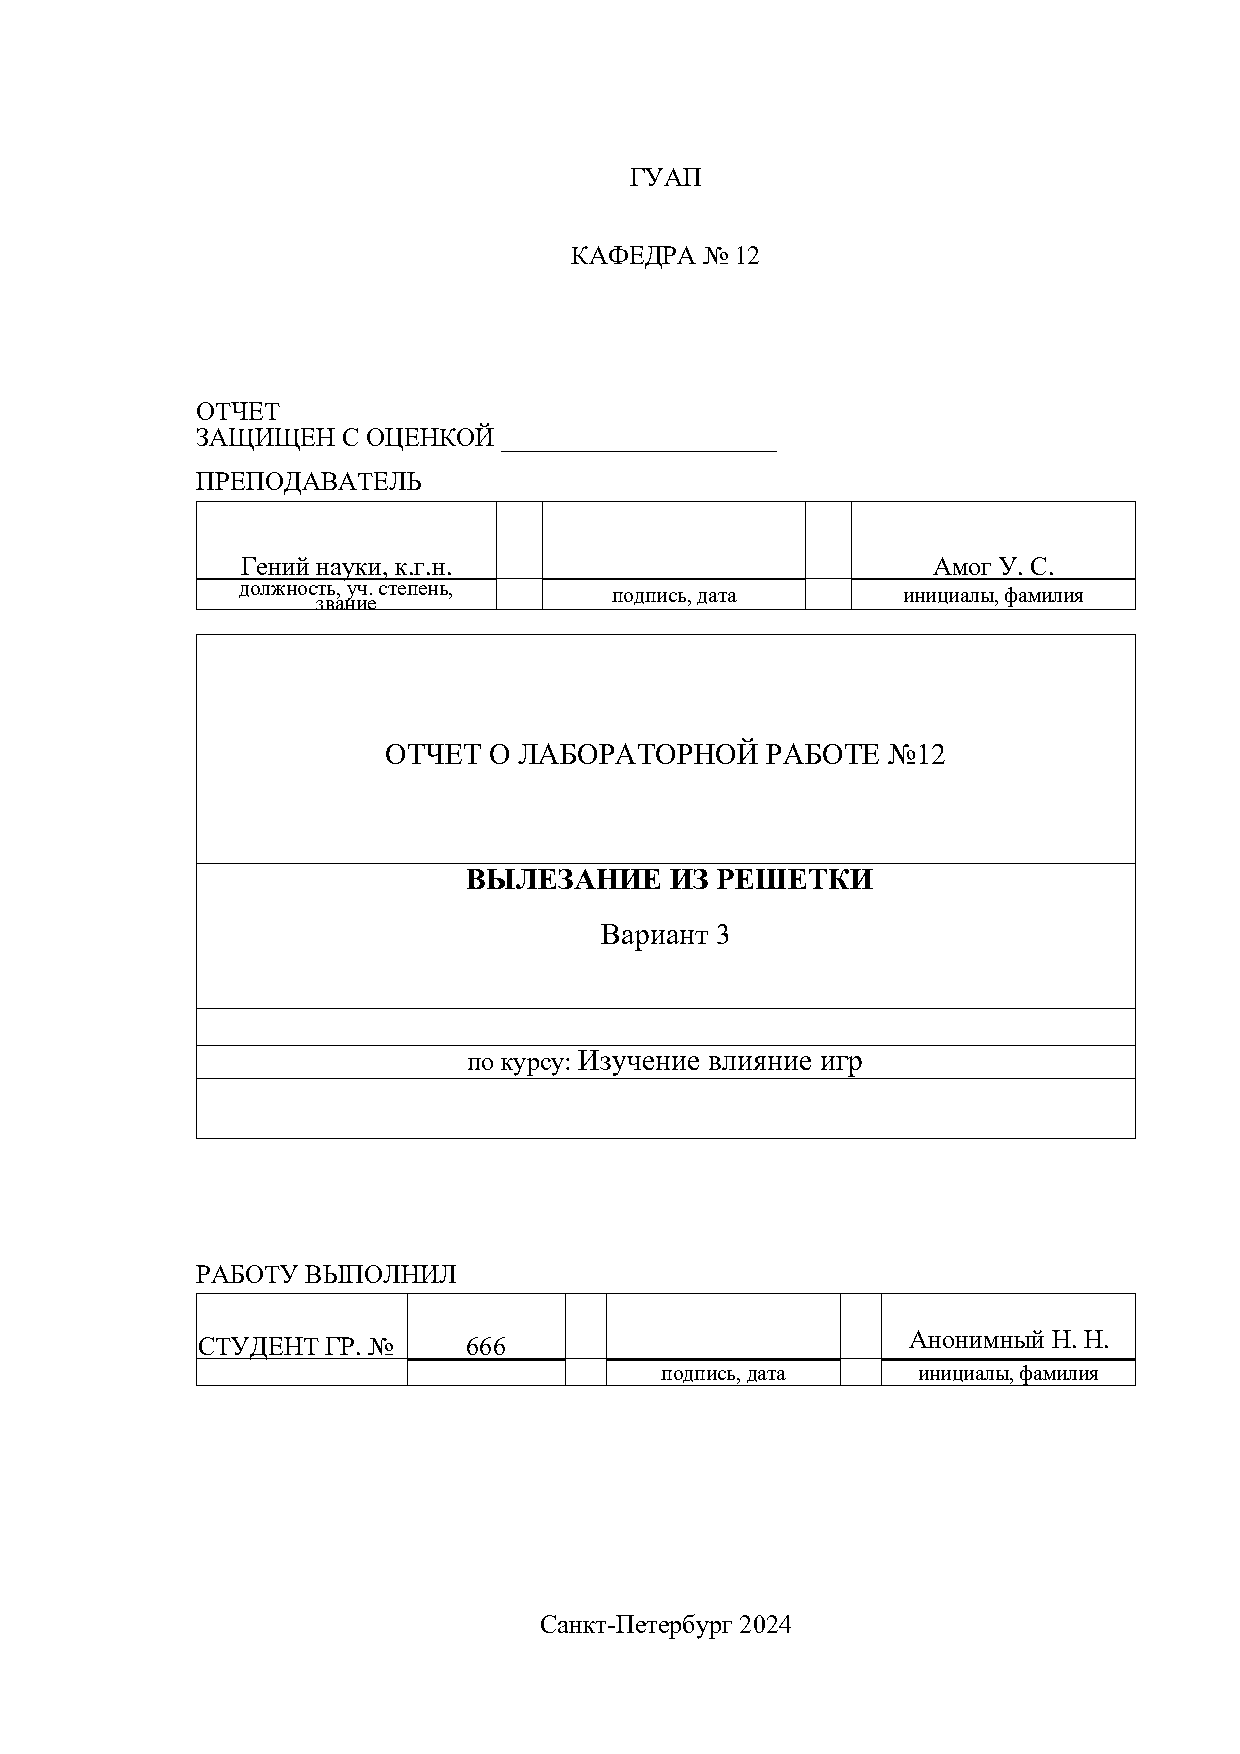
\includepdf[pages={1}, fitpaper=true]{\detokenize{/var/folders/mr/twkc4jg14f3cl5vr1lh0kgl80000gn/T/tmpyhcpm7q7/intro.pdf}}
\sloppy
\tableofcontents
\section{Почему suaidoc?}\label{ux43fux43eux447ux435ux43cux443-suaidoc}

suaidoc - это мощный инструмент для создания документации. Он
обеспечивает простоту использования, гибкость и мощные функции, которые
делают процесс создания документации более эффективным.

\subsection{Возможности}\label{ux432ux43eux437ux43cux43eux436ux43dux43eux441ux442ux438}

\begin{itemize}
\tightlist
\item
  Удобный CLI.
\item
  Генерация отчетов ГУАП из Markdown с использованием Pandoc.
\item
  Нумерация рисунков, формул и таблиц.
\item
  Соответствие ГОСТ 7.32 (За исключением таблиц)
\end{itemize}

\subsection{Как
установить?}\label{ux43aux430ux43a-ux443ux441ux442ux430ux43dux43eux432ux438ux442ux44c}

Установка suaidoc проста и быстра. Просто следуйте следующим шагам:

\begin{enumerate}
\def\labelenumi{\arabic{enumi}.}
\tightlist
\item
  Скачайте и установите последнюю версию suaidoc с официального сайта.
\item
  Откройте терминал и введите команду
  \passthrough{\lstinline!suaidoc --version!} чтобы убедиться, что
  установка прошла успешно.
\end{enumerate}

\section{Текст}\label{ux442ux435ux43aux441ux442}

\subsection{Параграфы}\label{ux43fux430ux440ux430ux433ux440ux430ux444ux44b}

Параграфы создаются также как и в Markdown. Параграфы, между которыми
нет пустой строки соединяются в один.

\subsubsection{Пустые
строки}\label{ux43fux443ux441ux442ux44bux435-ux441ux442ux440ux43eux43aux438}

В Markdown нельзя создавать пустые строки, но можно воспользоваться
\LaTeX.

Если требуется добавить 1 пустую строку, то нужно в конце параграфа
дописать \passthrough{\lstinline!\\newline!}.\newline

Текст спустя две строчки. \hfill \break \hfill \break

Или для нескольких пустых строк нужно написать
\passthrough{\lstinline!\\hfill \\break!}.

\subsection{Форматирование}\label{ux444ux43eux440ux43cux430ux442ux438ux440ux43eux432ux430ux43dux438ux435}

Поддержано все доступное форматирование текста в Markdown:

\begin{itemize}
\tightlist
\item
  \textbf{Жирный}
\item
  \emph{Курсив}
\item
  \textbf{\emph{Жирный курсив}}
\item
  \st{Перечеркнутый текст}
\end{itemize}

\subsection{Гиперссылки}\label{ux433ux438ux43fux435ux440ux441ux441ux44bux43bux43aux438}

Поддержаны гиперссылки из Markdown, но с оформлением по ГОСТ. Например,
ссылка на \href{https://github.com/vladcto/suaidoc}{репозиторий
\passthrough{\lstinline!suaidoc!}}.

В Markdown гиперссылках адрес может обрезаться на любом символе. Если
это поведение недопустимо, то нужно написать ссылку вручную.

\passthrough{\lstinline!название\_ссылки (URI - ссылка)!}

\subsection{Известные
проблемы}\label{ux438ux437ux432ux435ux441ux442ux43dux44bux435-ux43fux440ux43eux431ux43bux435ux43cux44b}

\textbf{1. Цитаты:}

На данный момент нет поддержки цитат, т.к. в ГОСТ нет каких-то
\emph{визуальных} требований к цитате.

\begin{quote}
Цитата отображается как обычный текст с меньшим отступом.
\end{quote}

\section{Заголовки}\label{ux437ux430ux433ux43eux43bux43eux432ux43aux438}

Поддержаны 3 уровня заголовков. Созданные заголовки автоматически
добавляются в оглавление.

\subsection{Заголовок 2
уровня}\label{ux437ux430ux433ux43eux43bux43eux432ux43eux43a-2-ux443ux440ux43eux432ux43dux44f}

\subsubsection{Заголовок 3
уровня}\label{ux437ux430ux433ux43eux43bux43eux432ux43eux43a-3-ux443ux440ux43eux432ux43dux44f}

Также можно задавать длинные заголовки. Слова перенесутся.

\subsection{Длинный заголовок - очень очень очень очень очень очень
очень очень очень очень очень длинный
заголовок}\label{ux434ux43bux438ux43dux43dux44bux439-ux437ux430ux433ux43eux43bux43eux432ux43eux43a---ux43eux447ux435ux43dux44c-ux43eux447ux435ux43dux44c-ux43eux447ux435ux43dux44c-ux43eux447ux435ux43dux44c-ux43eux447ux435ux43dux44c-ux43eux447ux435ux43dux44c-ux43eux447ux435ux43dux44c-ux43eux447ux435ux43dux44c-ux43eux447ux435ux43dux44c-ux43eux447ux435ux43dux44c-ux43eux447ux435ux43dux44c-ux434ux43bux438ux43dux43dux44bux439-ux437ux430ux433ux43eux43bux43eux432ux43eux43a}

\subsection{Известные
проблемы}\label{ux438ux437ux432ux435ux441ux442ux43dux44bux435-ux43fux440ux43eux431ux43bux435ux43cux44b-1}

\textbf{1. Ссылка на заголовок}

По умолчанию заголовки не имеют \passthrough{\lstinline!\\label!} при
экспорте из Markdown. Если вам потребуется сделать ссылку на заголовок,
то следует дописать \passthrough{\lstinline!\\label!} к заголовку, а
затем сослаться с помощью \passthrough{\lstinline!\\ref!}.

\begin{lstlisting}
# Я заголовок \label{section_name}

Хм, где мой заголовок \ref{section_name}.
\end{lstlisting}

\section{Списки}\label{ux441ux43fux438ux441ux43aux438}

\subsection{Ненумерованный
список}\label{ux43dux435ux43dux443ux43cux435ux440ux43eux432ux430ux43dux43dux44bux439-ux441ux43fux438ux441ux43eux43a}

\begin{itemize}
\item
  Ненумерованный поддержан за \emph{некоторыми} исключениями.
\item
  \(\mathit{Можно}\;\mathit{использовать}\;\mathit{формулы}\:\frac{1}{2}\).
\item
  Также можно писать длинные списки. Здесь текст списка занимает
  несколько строчек.
\item
  Список 1 уровня.

  \begin{itemize}
  \item
    Cписок 2 уровня.

    \begin{itemize}
    \tightlist
    \item
      Cписок 3 уровня. Cписок 2 уровня. Cписок 2 уровня. Cписок 2
      уровня. Cписок 2 уровня. Cписок 2 уровня.

      \begin{itemize}
      \tightlist
      \item
        Cписок 4 уровня. Глубже делать нельзя - ограничение LaTeX.
      \end{itemize}
    \end{itemize}
  \item
    Можно начать текст с новой строки.

    Нужно не следующем уровне табуляции начать писать текст.
  \end{itemize}
\end{itemize}

\subsection{Нумерованный
список}\label{ux43dux443ux43cux435ux440ux43eux432ux430ux43dux43dux44bux439-ux441ux43fux438ux441ux43eux43a}

\begin{enumerate}
\def\labelenumi{\arabic{enumi}.}
\item
  \(\mathit{Можно}\;\mathit{использовать}\;\mathit{формулы}\:\frac{1}{2}\).
\item
  Также можно писать длинные списки. Здесь текст списка занимает
  несколько строчек.
\item
  Можно начать текст с новой строки

  Можно начать текст с новой строки.
\end{enumerate}

\subsection{Известные
проблемы}\label{ux438ux437ux432ux435ux441ux442ux43dux44bux435-ux43fux440ux43eux431ux43bux435ux43cux44b-2}

\textbf{1. Нумерованный список не может иметь подсписки}

Это ограничение Markdown, нумерованных вложенных списков не существует в
Markdown.

Можно использовать \LaTeX:

\begin{enumerate}
\item первый элемент первого уровня содержит список
\begin{enumerate}
\item элемент списка второго уровня
\item второй элемент списка второго уровня
\end{enumerate}
\item второй элемент первого уровня
\end{enumerate}

\section{Изображения}\label{ux438ux437ux43eux431ux440ux430ux436ux435ux43dux438ux44f}

\subsection{Вставка}\label{ux432ux441ux442ux430ux432ux43aux430}

Вставка изображений в suaidoc осуществляется с помощью следующего
синтаксиса: \passthrough{\lstinline"!­[альтернативный текст](URL)"}.
Альтернативный текст будет отображаться, если изображение не может быть
загружено.

\image{report_images/image.png}{Пример изображения}{0.95}

\subsection{Изменение
размера}\label{ux438ux437ux43cux435ux43dux435ux43dux438ux435-ux440ux430ux437ux43cux435ux440ux430}

Для изменения размера нужно указать размер после ссылки в
\passthrough{\lstinline!<>!}. Размер указывается в проценте заполнения
ширины страницы.

\begin{lstlisting}
!­[Логотип](https://example.com/logo.png)<l>
\end{lstlisting}

Изображение масштабируется сохраняя пропорции. На таблице \ref{1}
изображены значения тегов.

\begin{longtable}[]{@{}cc@{}}
\caption{ширина тегов \label{1}}\tabularnewline
\toprule\noalign{}
Тег & \% ширины \\
\midrule\noalign{}
\endfirsthead
\toprule\noalign{}
Тег & \% ширины \\
\midrule\noalign{}
\endhead
\bottomrule\noalign{}
\endlastfoot
l & 85 \\
m & 55 \\
sm & 35 \\
t & 25 \\
\end{longtable}

\image{report_images/image-1.png}{Изображение с sm}{0.35}

\subsection{Ссылки на
изображения}\label{ux441ux441ux44bux43bux43aux438-ux43dux430-ux438ux437ux43eux431ux440ux430ux436ux435ux43dux438ux44f}

Для ссылки на изображение достаточно указать то, что было указано для
\emph{alt text} (\passthrough{\lstinline"!­[alt-text]..."}) в
\passthrough{\lstinline!\\ref\{fig:alt-text\}!}.

Например ссылка на рисунок \ref{fig:Изображение с sm}.

\section{Формулы}\label{ux444ux43eux440ux43cux443ux43bux44b}

В Markdown можно ставить формулы располагая их внутри \emph{долларов}.
Сами же формулы пишутся с использованием \LaTeX. Можно использовать
русские символы в формулах, но они будут написаны курсивом основного
шрифта.

\begin{equation}\begin{gathered}

\mathbf{A} = 
\begin{bmatrix}
a_{11} & a_{12} \\
a_{21} & a_{22} \\
\end{bmatrix}, \quad
\mathbf{A}^T = 
\begin{bmatrix}
a_{11} & a_{21} \\
a_{12} & a_{22} \\
\end{bmatrix}
,\;\mathit{как}\;\mathit{пример}

\label{eq:Пример}
\end{gathered}\end{equation}

\subsection{Нумерация}\label{ux43dux443ux43cux435ux440ux430ux446ux438ux44f}

Для нумерации: \begin{equation}
\begin{gathered}2+2=5\end{gathered}
\end{equation}

\subsection{Ссылки на
формулы}\label{ux441ux441ux44bux43bux43aux438-ux43dux430-ux444ux43eux440ux43cux443ux43bux44b}

Для создания ссылок на формулы используйте тег AOAOAO внутри формулы. а
затем используйте \passthrough{\lstinline!\\ref\{eq:имя\_формулы\}!}.

\section{Таблицы}\label{ux442ux430ux431ux43bux438ux446ux44b}

\subsection{Написание}\label{ux43dux430ux43fux438ux441ux430ux43dux438ux435}

Таблицы в Markdown создаются с использованием вертикальных и
горизонтальных линий. Вертикальные линии \passthrough{\lstinline!|!}
используются для разделения столбцов, а горизонтальные
\passthrough{\lstinline!-!} для разделения заголовка таблицы от ее
содержимого.

\subsection{Вариации}\label{ux432ux430ux440ux438ux430ux446ux438ux438}

Вы можете выравнивать текст в столбцах по левому краю, по правому краю
или по центру, используя соответствующие символы в строке, разделяющей
заголовок и содержимое таблицы.

\subsection{Таблица из
файла}\label{ux442ux430ux431ux43bux438ux446ux430-ux438ux437-ux444ux430ux439ux43bux430}

Вы можете включить таблицу из файла, используя синтаксис включения
файлов Markdown. Просто укажите путь к файлу в круглых скобках после
ключевого слова \passthrough{\lstinline!include!}.

\subsection{Ссылки на
таблицы}\label{ux441ux441ux44bux43bux43aux438-ux43dux430-ux442ux430ux431ux43bux438ux446ux44b}

Для создания ссылок на таблицы используйте тег
\passthrough{\lstinline![текст ссылки](\#идентификатор-таблицы)!}.
Идентификатор таблицы - это текст заголовка таблицы, преобразованный в
нижний регистр и замененный пробелы на дефисы.

\subsection{Известные
проблемы}\label{ux438ux437ux432ux435ux441ux442ux43dux44bux435-ux43fux440ux43eux431ux43bux435ux43cux44b-3}

Некоторые редакторы Markdown могут не поддерживать все возможности
форматирования таблиц. В частности, могут быть проблемы с поддержкой
вложенных таблиц, таблиц с многострочными ячейками и таблиц с ячейками,
содержащими списки или другие элементы форматирования.

\section{Код}\label{ux43aux43eux434}

\subsection{Inline код}\label{inline-ux43aux43eux434}

Для вставки коротких фрагментов кода в текст используйте обратные
кавычки (`). Обратные кавычки обозначают начало и конец фрагмента кода.
Внутри обратных кавычек код будет отображаться моноширинным шрифтом и
будет отделен от остального текста.

\subsection{Оформление
листинга}\label{ux43eux444ux43eux440ux43cux43bux435ux43dux438ux435-ux43bux438ux441ux442ux438ux43dux433ux430}

Для вставки больших блоков кода используйте тройные обратные кавычки
(```). Вставьте код между двумя строками, каждая из которых состоит из
трех обратных кавычек. Код внутри такого блока будет отображаться
моноширинным шрифтом и будет отделен от остального текста. Вы также
можете указать язык программирования сразу после открывающих кавычек,
чтобы включить подсветку синтаксиса.

\subsection{Листинг из
файла}\label{ux43bux438ux441ux442ux438ux43dux433-ux438ux437-ux444ux430ux439ux43bux430}

Вы можете включить код из файла, используя синтаксис включения файлов
Markdown. Просто укажите путь к файлу в круглых скобках после ключевого
слова \passthrough{\lstinline!include!}. Код из файла будет вставлен в
документ и отформатирован как блок кода.
\end{document}
